% !TEX root = ../thesis.tex
\iffalse
Results

    The results are actual statements of observations, including statistics, tables and graphs.
    Indicate information on range of variation.
    Mention negative results as well as positive. Do not interpret results - save that for the discussion. 
    Lay out the case as for a jury. Present sufficient details so that others can draw their own inferences and construct their own explanations. 
    Use S.I. units (m, s, kg, W, etc.) throughout the thesis. 
    Break up your results into logical segments by using subheadings
    Key results should be stated in clear sentences at the beginning of paragraphs.  It is far better to say "X had significant positive relationship with Y (linear regression p<0.01, r^2=0.79)" then to start with a less informative like "There is a significant relationship between X and Y".  Describe the nature of the findings; do not just tell the reader whether or not they are significant.  
\fi


\section{Pruning}
In this section we consider the configurations that have pruned the most nodes as our results. Since the combination of variables and parameters that we have used are very big, we chose not to report the configurations that are not working. 

As we have explained in Chapter~\ref{cha:methods}, we have pruned the nodes of a fully connected neural network trained to predict the summation of two floating point values, and an autoencoder trained on the MNIST dataset. We ran the experiments at least three times with each configuration to verify our results.

\subsection{Fully Connected Networks}
We have initialized and run training cycles on the fully connected network. By applying distortions to remaining weights between training cycles, we have achieved the optimum result we have shown in Figure~\ref{fig:optimum_fc_summation}, with only one node in the hidden layer. 

When distortions were applied between training cycles, both pruning criteria worked equally good. For both criteria, we were able to achieve the optimum network structure using a fixed threshold of $0$. In other words, for activation count criteria, we have pruned the nodes that were not being activated, and for activation variance criteria, we have pruned the nodes that had zero variance in values.

The loss was almost zero for the training and test datasets. Even though we have achieved the optimal shape, the model was overfitting for the mean and standard deviation parameters we set for the random number generator while generating the training dataset.

In the experiments that we did not apply distortions, we could not find a configuration that achieves the optimal network structure. In most of the configurations we were unable to find any nodes to prune after the first training cycle. We could not see any difference between different regularization terms or pruning criteria.

\subsection{Convolutional Neural Networks}
In this setting using activation variance criterion and L2 regularization, we have achieved the most optimum result. We did not see any improvement by using distortions. Using L2 regularization, compared to no regularization and L1 regularization, we have seen an improvement in the number of nodes pruned in every training cycle and the final result.

We were unable to find a good threshold for activation count criterion. However, doing a basic outlier selection with the activation variances worked best. Given that $v$ is the variance vector each output feature of a layer, by choosing a lower and upper boundaries as,
$$ mean(v) - 2*var(v) < x < mean(v) + 2*var(v) $$
and removing the nodes that are not outside these boundaries, we were able to find the most optimum solutions. 

The most ideal case was with no distortion, L2 regularization (with $\lambda = 0.01$) and pruning nodes based on activation variance criterion given above. Using this setting, we have pruned the autoencoder from $1-32-64-32-1$ to $1-2-4-3-1$ nodes per layer, which is a much better result compared to the baseline we have defined. It took us $10\pm4$ training cycles to achieve this result. The loss we have achieved is very close to 0. The encoder we have achieved is shown in Figure~\ref{fig:pruned_autoencoder}.
\begin{figure}[!h]
    \begin{subfigure}{1\textwidth}
        \hspace{-.1\linewidth}
        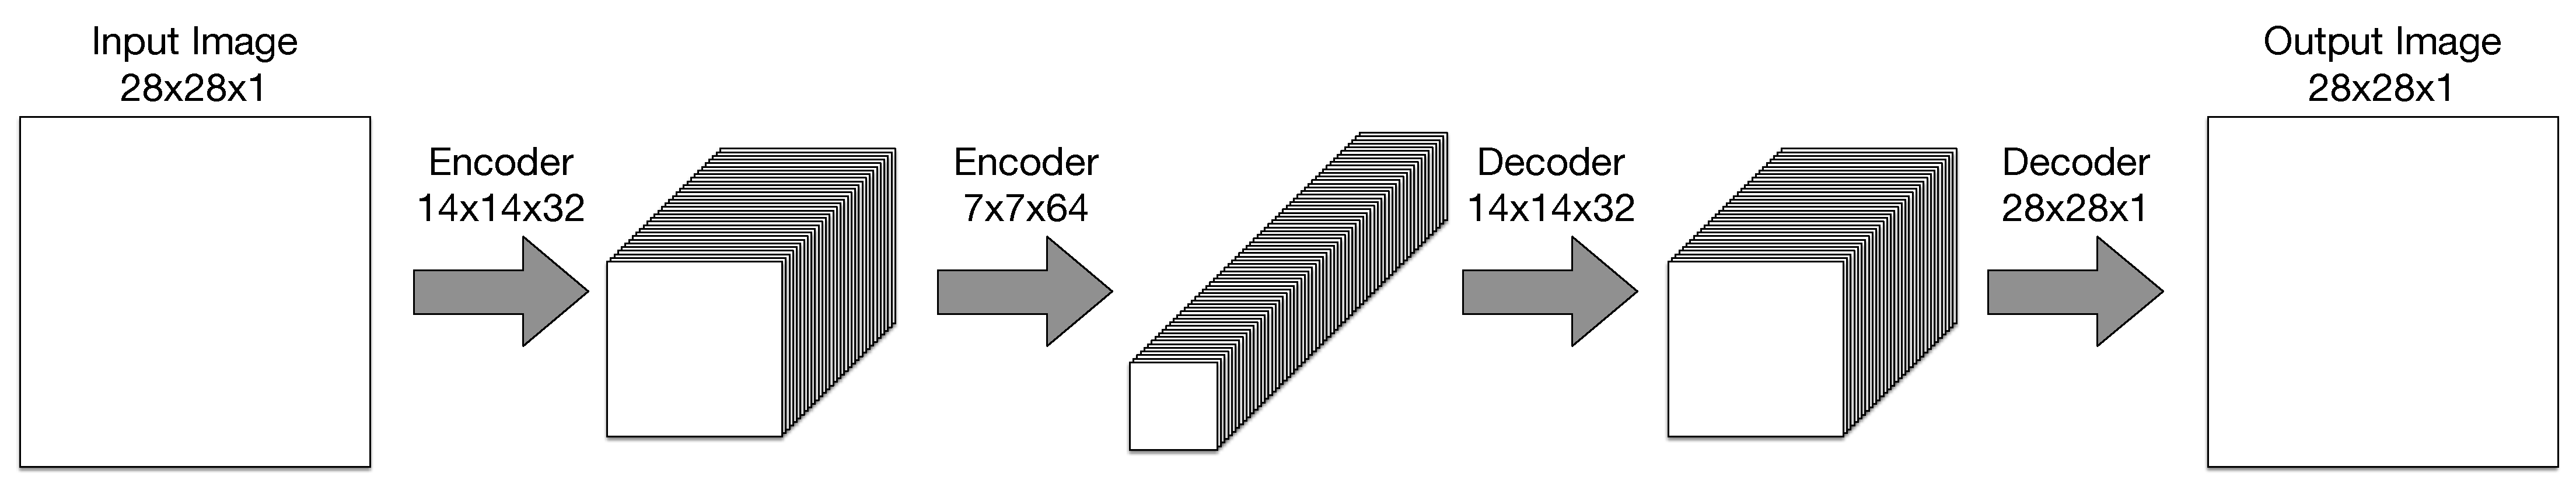
\includegraphics[width=1.2\linewidth]{images/over_parameterized_autoencoder.pdf}
        \caption{Initial autoencoder configuration.}
        \label{fig:initial_autoencoder}
    \end{subfigure}
    \begin{subfigure}{1\textwidth}
        \hspace{-.1\linewidth}
        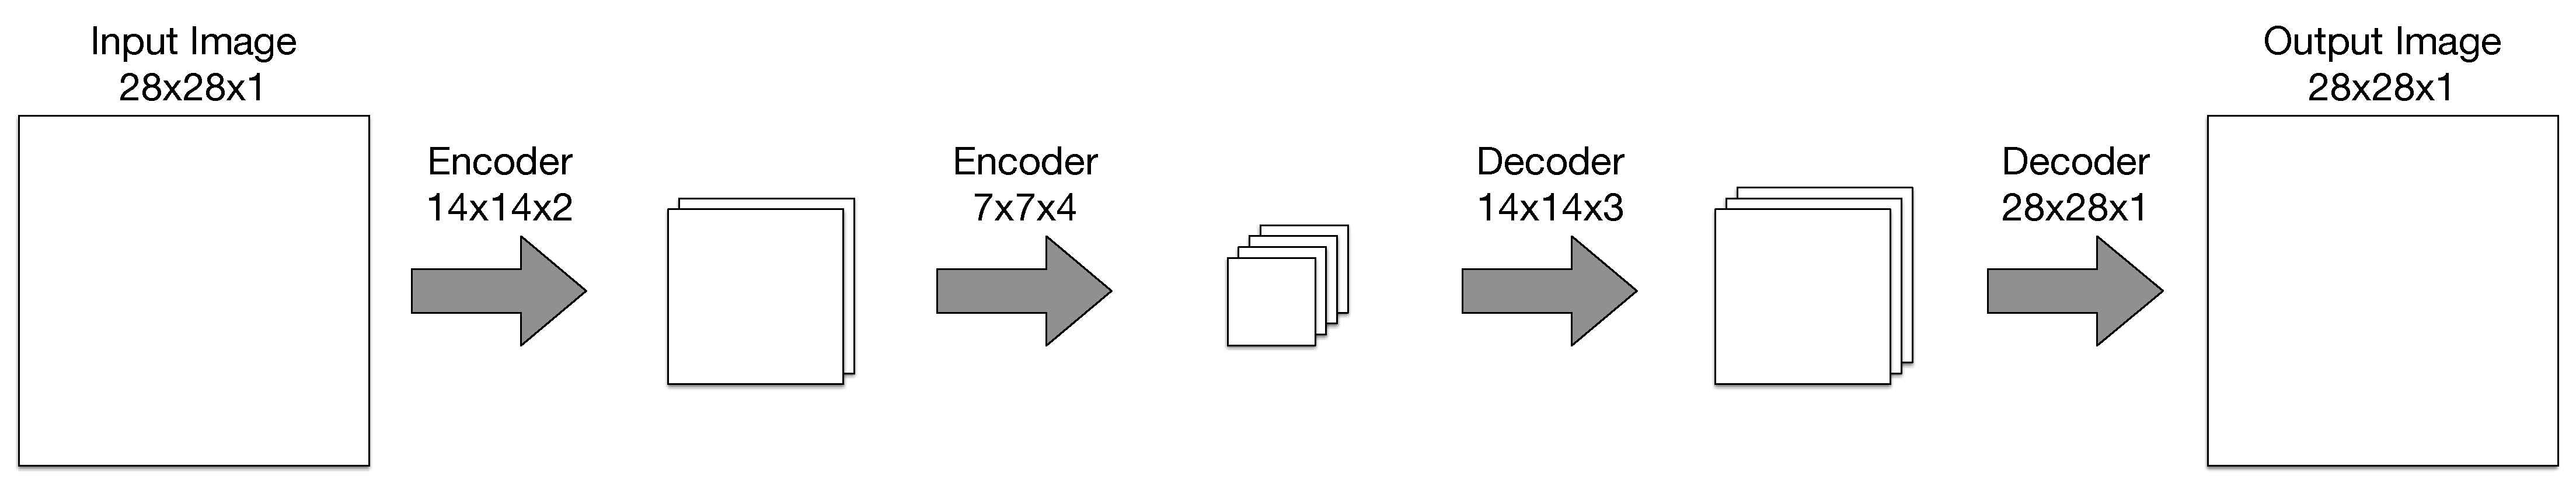
\includegraphics[width=1.2\linewidth]{images/optimum_autoencoder.pdf}
        \caption{Resulting autoencoder configuration.}
        \label{fig:pruned_autoencoder}
    \end{subfigure}
    \caption{Pruned autoencoder compared to initial autoencoder.}
    \label{fig:pruned_autoencoder}
\end{figure}

\newpage
\section{Convolution Operation Alternatives}
We ran experiments to see which operation is could be an alternative to convolution operation. We ran our experiments 10 times to validate our results. We compare these results in terms of accuracy.
\subsection{MNIST}
In our experiments with MNIST dataset, we have not seen a comparable difference between experiments with different operations. All of the experiments have resulted with $99\pm0.3\%$ top-1 accuracy, with no clearly visible difference in terms of accuracy.
\subsection{CIFAR-10}
The results of our experiments in CIFAR-10 dataset are given in Table~\ref{tab:convolution_alternative_results}.
\begin{table}[]
\centering
\begin{tabular}{| l | r | r | r |}
\thead{Model}                                                                     & \thead{Mean accuracy} & \thead{Max accuracy}  & \thead{Ops} \\ \hline
Convolution (baseline)                                                             & 81.84                  & 82.56        & 16.1~M         \\ \hline
Kernel composing conv.                                                             & 81.98                  & 82.51      & 8~M           \\ \hline
Separable convolution                                                              & 82.11                  & 82.53        & \textbf{2.1~M}         \\ \hline
\begin{tabular}[c]{@{}l@{}}Separable convolution\\ with non-linearity\end{tabular} & \textbf{82.16}         & \textbf{82.75}   & \textbf{2.1~M}     \\ \hline
\end{tabular}
\caption{Mean and max of top-1 accuracy results, using CIFAR-10 validation dataset and number of operations for each model.}
\label{tab:convolution_alternative_results}
\end{table}
As emphasized in the table, separable convolution operation with non-linearity performed slightly better than the rest of the operations. The models that use separable convolutions require 8 times fewer operations than the baseline and almost 4 times fewer operations than the kernel composing convolution operation. To validate our results, we ran each experiment 10 times.

\section{Small Models}
In this section we will present the results of our experiments on small models. We show how small models perform compared to large ones and see how pruning and approximation methods work with them.
\subsection{Models}
\label{sec:result_models}
\subsubsection{CIFAR-10}
The model we have defined for this task (see Figure~\ref{fig:separable_resnet_cifar10}), has achieved a maximum of 91.1\% top-1 classification accuracy on CIFAR-10 test dataset in 10 training sessions. As we have shown in Table~\ref{tab:cifar-model-vs-resnet-20}, compared to ResNet-20 (\cite{He:2015aa}), our model has performed slightly worse in terms of top-1 classification accuracy. However, in terms of floating point operations and number of parameters, our model is about 2 times smaller in terms of number of parameters, and requires 4 times fewer floating point operations to perform an inference.

\begin{table}[!h]
\hspace{-21px}
\begin{tabular}{|l|r|r|r|r|r|r|}
\thead{Model} & \thead{Params} & \thead{Layers} & \thead{Blocks} & \thead{Ops}  & \thead{Size} & \thead{Top-1 ac. (\%)} \\ \hline
Our Model                          & $\mathbf{0.12~M}$               & $27$  & $6$                & $\mathbf{\sim 13~M}$ & $\mathbf{581 KB}$             & 91.10                        \\ \hline
ResNet-20                          & $0.27$ M               & $20$ & $9$                 & $\sim$ $40$ M & $ 1109 $KB           & $\mathbf{91.25}$                        \\ \hline
\end{tabular}
\caption{Our small model compared with ResNet-20 from \cite{He:2015aa}.}
\label{tab:cifar-model-vs-resnet-20}
\end{table}

\subsubsection{ImageNet}
The model we have defined for this task (see Figure~\ref{fig:model}), has achieved a maximum of 63 \% top-1 classification accuracy on ImageNet test dataset. We trained this model only once. Compared to ResNet-34 (\cite{He:2015aa}), which is reported to achieve $73.1\%$ top-1 classification accuracy\footnote{\url{http://torch.ch/blog/2016/02/04/resnets.html}}, our model has performed badly.

\subsection{Pruning Small Models}
\label{sec:pruning_small_models}
Using the pruning criteria we have defined for autoencoders, we have tried to prune the CIFAR-10 model. However, we were unable find a configuration that prunes a significant amount of nodes and recover the accuracy in the next training cycle. 

\subsection{Approximating Small Models}
\label{sec:approximating_small_models}
We ran the approximation tool we have defined on our best model (91.1 \% top-1 accuracy) from our CIFAR-10 experiments. Using various pruning thresholds and error thresholds, we could not find any factorization that would make this model faster while preserving the accuracy.

\subsection{Quantization}
\label{sec:quantizing_small_models}
We have quantized the CIFAR-10 model, converting 32-bit floating point operations to 8-bit floating point operations. However, in our benchmarks, we have seen that this method has slowed down the inference speed by almost half. We haven't seen any significant change in the model accuracy.

\iffalse
\section{Benchmarks and Comparisons}
We have benchmarked 20 models in different sizes and shapes using our benchmarking device. Here we will report the models that we found important.

Inception-Resnet-v2 (\cite{DBLP:journals/corr/SzegedyIV16}) has a model size of 224 MB and our benchmarking device could execute 0.3-0.4 inferences per second. The cpu-utilization with this model was 0.006568. On a 4 core device, this number is extremely low, so we can conclude this model is cursed by the memory bottleneck bandwidth. 

We have seen that ResNet-50 (\cite{He:2015aa}, \cite{he2016identity}) with a model size of 100 MB got executed for 1.3-1.7 inferences per second with a cpu-utilization of 2.7. We found this amount to be great compared to the previous model.  

Among many models we have inspected, only 1.0 MobileNet-224 (\cite{howard2017mobilenets}) performed faster than our separable resnet. 1.0 Mobilenet-224 had a model size of 17.1 MB and our benchmarking device could perform 5 to 6 inferences per second with a cpu-utilization of 2.7. 

\begin{table}[!h]
\hspace{-30px}
\label{my-label}
\begin{tabular}{|l|r|r|r|r|r|}
\thead{\small Model}      & \thead{\small top-1 ac.(\%)} & \thead{\small \# layers}                                                          & \thead{\small model size} & \thead{\small cpu util.} & \thead{\small inf./sec.} \\ \hline
Inception-resnet-v2 & 80.1 & \textbf{131}                                                                                                  & 224 MB                      & \textbf{0.006}                    & 0.35                      \\ \hline
ResNet-50           & 75.9\footnote{\url{https://github.com/facebook/fb.resnet.torch/blob/master/pretrained/README.md}}  & 50 & 100 MB                      & 2.7                      & 1.5                       \\ \hline
1.0 Mobilenet-224   & 70.6        &    28                                                                                       & 17.1 MB                     & 2.7                      & \textbf{5.5}                       \\ \hline
Our ImageNet Model  & 63         & 77                                                                                           & 12.1 MB                      & 3.1                      & 4.5                      \\ \hline
\end{tabular}
\caption{Benchmark results for various models.}
\end{table}
\fi
